\documentclass{article}

% NeurIPS 2025 style, used for layout only. The preprint option prints "Preprint."
% in the footer. This report has not been submitted to or reviewed by NeurIPS.
\usepackage[preprint,nonatbib]{neurips_2025}

% Compiled with a XeTeX-based engine (tectonic), so the Times text face the
% style expects is loaded through fontspec. Math stays in Computer Modern.
\usepackage{fontspec}
\setmainfont{texgyretermes}[Extension=.otf, UprightFont=*-regular, BoldFont=*-bold, ItalicFont=*-italic, BoldItalicFont=*-bolditalic]
\setsansfont{texgyreheros}[Extension=.otf, UprightFont=*-regular, BoldFont=*-bold, ItalicFont=*-italic, BoldItalicFont=*-bolditalic, Scale=MatchLowercase]

\usepackage{amsmath}
\usepackage{booktabs}
\usepackage{graphicx}
\usepackage{xcolor}
\usepackage{tikz}
\usetikzlibrary{arrows.meta,positioning}
\usepackage[hidelinks]{hyperref}
\usepackage{url}

\definecolor{accent}{HTML}{B4532F}
\definecolor{ink}{HTML}{1B1B1A}
\definecolor{faint}{HTML}{8B8882}
\definecolor{rule}{HTML}{D8D4CD}
\definecolor{panel}{HTML}{F3F1ED}

\newcommand{\code}[1]{\texttt{\small #1}}

\title{Orbifex: Synthetic Workspaces from a Persona,\\ with Answer-Preserving Complexity Tiers}

\author{%
  Neal Desai \\
  Independent \\
  \url{https://nealdes.ai}
}

\begin{document}

\maketitle

\begin{abstract}
Agents that work over a person's mail, calendar, files and apps are hard to evaluate because the environments are private, the right answers are rarely recorded, and difficulty labels are usually assigned by the author and never measured. We describe Orbifex, a generator that turns a short persona description into a seeded workspace with eight data sources, three of the persona's own and five exported from third-party apps, and a set of questions whose answers are computed before any text is rendered. Final facts are drawn from random streams that do not depend on the complexity tier, so a question keeps one answer while the workspace grows from 59 files to 4{,}225. Every answer must then be recovered from the rendered files by an independent solver, and each task is exported as a self-contained Harbor task. On one persona at four tiers (188 tasks), a small model with file-search tools answered 242 of 252 runs correctly. Growing the workspace 141-fold raised cost and barely changed accuracy. Eight of the ten errors came from one kind of question, asked for two months, and reproduce a wrong answer the generator had predicted, the one implied by an invoicing-app export that is out of date because a due-date extension agreed over email never reached it. Deleting that export restored 12 of 12 answers. An earlier version of the workspace without the export had already produced the same wrong answer in 2 of 12 runs, because the invoices and a tracker spreadsheet carry the old dates as well, so the export raised the error rate and is not its only source. Running the exported archive end to end also exposed a container-build fault that graded tasks against another task's answer key. We describe its cause, a fix, and a static check for it.
\end{abstract}

\section{Introduction}

A useful evaluation of an assistant that reads someone's mailbox needs three things that are difficult to obtain together. The environment has to look like a real working life, with several sources that describe the same events. The answer to each question has to be known with certainty. And the difficulty of a task has to be something the author can state and defend. Real workspaces offer the first and forbid the other two, since they are private and nobody wrote the answers down. Synthetic workspaces can offer all three, provided the generator is built around the answers and the difficulty claims are checked.

Recent systems build environments from a persona \cite{wildawm,mypcbench}, compile tasks from a single specification so that instruction, environment and verifier cannot disagree \cite{anchor}, and scale an environment while holding answers fixed \cite{enterprisebench}. A recurring finding in this literature is that difficulty labels set by construction do not survive measurement. EmailBench reports that its level labels ``are metadata rather than experimentally calibrated difficulty levels'' and that results ``are not monotonic across them'' \cite{emailbench}. One synthetic-environment pipeline therefore accepts a task into a tier only when a reference model's pass rate lands inside that tier's band \cite{generalagent}, and GRADS observes that evidence added to raise difficulty ``may be only weakly coupled to the answer, creating a mismatch between intended and empirical difficulty'' \cite{grads}.

This report describes a small generator built with those findings in mind and then tests whether its own tiers hold up. The contributions are as follows.

\begin{itemize}
  \item A generator in which the final value of every fact is drawn independently of the complexity tier, so the same question has the same answer at every tier while history, look-alike entities and volume grow around it (Section~\ref{sec:method}).
  \item A set of export gates centred on an independent solver that must recover each answer from the rendered files, plus a claims manifest that ties every rendered unit to the facts it states (Section~\ref{sec:gates}).
  \item A pilot on 188 tasks in which a 141-fold increase in workspace size barely changed a small agent's accuracy, while accuracy on the two questions touched by an authoritative-looking source that lags behind the truth was 4 of 12, against 12 of 12 when that source alone is deleted and 10 of 12 in an earlier version that lacked it (Section~\ref{sec:results}).
  \item A description of a container-build fault that silently grades a task against another task's key, found only by running the published archive, with a fix and a static check (Section~\ref{sec:fault}).
\end{itemize}

\section{Related work}

\paragraph{Persona-first environments.} WildAWM has a coding agent write a persona, plan it day by day and materialise each day as a replayable program, and filters tasks through execution gates that include solvability and a counterfactual probe \cite{wildawm}. MyPCBench drives deterministic seeders for 17 applications from one persona file and grades 184 tasks with a rubric-based model judge \cite{mypcbench}. Orbifex is far smaller in scope. It differs in keeping grading free of model judges and in treating the complexity tier as an experimental variable with the answer held fixed.

\paragraph{Single-source task construction.} Anchor compiles the instruction, environment, oracle and verifier of each task from one parametric specification to prevent what its authors call artifact drift, releases its tasks in Harbor format, and checks each with a no-op and an oracle replay \cite{anchor}. We follow the same discipline and add a second, independent derivation of each answer from the files the agent will see.

\paragraph{Scale with the answer held fixed.} Enterprise-Bench describes an ``answer-preserving dataset design'' that holds the correct answer constant within a production-scale volume of noise \cite{enterprisebench}. Our tiers apply that idea to a personal workspace and add superseded versions of the queried facts, which is a different kind of pressure from unrelated volume.

\paragraph{Calibrated difficulty.} Beyond the results cited above \cite{emailbench,generalagent,grads}, the general lesson is that a difficulty label is a hypothesis until a solver's pass rate supports it. Our pilot is a small instance of that test applied to our own tiers.

\paragraph{Benchmark integrity and task formats.} Audits of agent benchmarks have found large numbers of exploitable flaws, including an automated auditor that reported 219 distinct flaws across ten benchmarks and reached near-perfect scores on most ``without solving a single task'' \cite{benchjack}, and a study that found 16\% of 1{,}968 terminal-agent tasks hackable by frontier models \cite{hackerfixer}. Harbor packages a task as a directory with an instruction, an environment, tests and an optional reference solution, and since 2026 can run the verifier in a sandbox separate from the agent's \cite{harbor}. We export to that format and report a failure mode of the separate-verifier build path.

\section{Method}
\label{sec:method}

\begin{figure}[t]
  \centering
  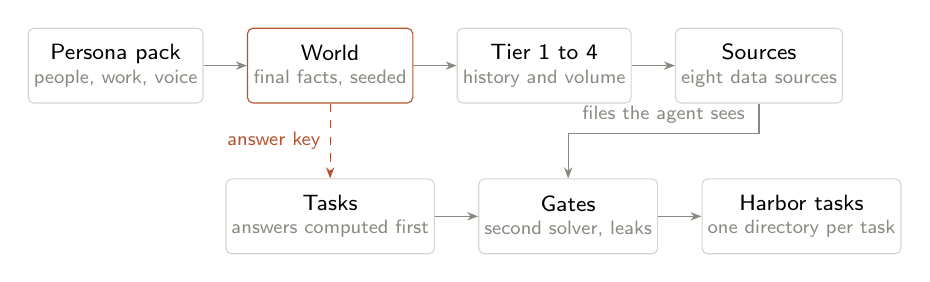
\begin{tikzpicture}[font=\sffamily\footnotesize, >={Stealth[length=4pt]},
      box/.style={draw=rule, rounded corners=2pt, minimum width=2.1cm, minimum height=0.95cm, align=center, inner sep=2pt},
      hot/.style={box, draw=accent}]
    \node[box] (pack) {Persona pack\\[-1pt]{\scriptsize\color{faint}people, work, voice}};
    \node[hot, right=0.55cm of pack] (world) {World\\[-1pt]{\scriptsize\color{faint}final facts, seeded}};
    \node[box, right=0.55cm of world] (tier) {Tier 1 to 4\\[-1pt]{\scriptsize\color{faint}history and volume}};
    \node[box, right=0.55cm of tier] (src) {Sources\\[-1pt]{\scriptsize\color{faint}eight data sources}};
    \node[box, below=0.95cm of world] (tasks) {Tasks\\[-1pt]{\scriptsize\color{faint}answers computed first}};
    \node[box, right=0.55cm of tasks] (checks) {Gates\\[-1pt]{\scriptsize\color{faint}second solver, leaks}};
    \node[box, right=0.55cm of checks] (harbor) {Harbor tasks\\[-1pt]{\scriptsize\color{faint}one directory per task}};
    \draw[->, faint] (pack) -- (world);
    \draw[->, faint] (world) -- (tier);
    \draw[->, faint] (tier) -- (src);
    \draw[->, accent, dashed] (world) -- node[left, font=\sffamily\scriptsize, text=accent] {answer key} (tasks);
    \draw[->, faint] (tasks) -- (checks);
    \draw[->, faint] (checks) -- (harbor);
    \draw[->, faint] (src.south) |- ++(0,-0.38) -| node[pos=0.25, above, font=\sffamily\scriptsize, text=faint] {files the agent sees} (checks.north);
  \end{tikzpicture}
  \caption{The pipeline. The answer key is computed from the world model. The gates then require a separate solver to reach the same answers from the rendered files alone.}
  \label{fig:pipeline}
\end{figure}

Figure~\ref{fig:pipeline} shows the pipeline. The implementation is 2{,}242 lines of Python with no dependencies outside the standard library.

\subsection{Persona pack}

A persona pack is a TOML file of about 300 lines (329 for the accountant and 292 for the designer). It names the persona and an assistant, lists the organisations they deal with, gives the vocabulary of the work (what an engagement cycle, a deliverable and a meeting are called), and supplies a voice profile of openers, closers and stock reasons for rescheduling or correcting something. Two packs exist, a solo accountant who closes the books for small businesses each month and an independent brand designer on monthly retainers. Both share one engine that models a monthly cycle of request, documents, meeting, invoice and payment.

\subsection{Tier-invariant facts}

Let a fact be identified by an entity $e$, a month $m$ and a field $f$, such as the due date of one client's April invoice. Its final value is
\begin{equation}
  v(e, m, f) = g_f\bigl(\mathrm{RNG}(s, e, m)\bigr),
\end{equation}
where $s$ is the seed and $g_f$ draws the field from a stream keyed only by $(s, e, m)$. The tier $\tau \in \{1,2,3,4\}$ never enters this draw. A tier instead controls three other things, each drawn from separate streams. It sets how many superseded versions precede the final value of a fact (a meeting that moved twice, an invoice corrected twice, a due date that was extended). It sets how many additional entities exist, including look-alike organisations whose names collide with the core ones. And it sets volume, meaning months of history, unrelated mail, calendar clutter and Slack chatter.

The consequence is a property we test directly. For every fact about the three core clients in the two core months, the final value is identical at all four tiers. A unit test builds the world for 20 seeds at each tier and asserts this equality, and a second test asserts that the same seed yields a byte-identical workspace archive.

\subsection{Sources, rendering and the claims manifest}
\label{sec:sources}

Three sources are the persona's own. Mail is written as plain \code{.eml} files with threading headers and CSV attachments, the calendar as a single \code{.ics} file whose events carry sequence numbers and cancellations, and the drive as a tree of files that includes a tracker spreadsheet. Five more are exports from third-party apps. A Slack workspace is written in Slack's export layout, with \code{users.json}, \code{channels.json} and one file per channel per day. The bank provides monthly statement exports in which client payments, card purchases and refunds all post. An invoicing app exports its invoices and payments, a time tracker its hours per project, and a retailer its order history and refunds.

Each event is rendered into every source that would plausibly record it. An invoice correction produces a message in the sent-mail folder, a revised file in the drive, a Slack remark and a new total in the invoicing app, and the earlier versions remain where they were. Each app therefore holds its own copy of some facts. The bank, the time tracker and the order history agree with the final truth, and the Slack export is a running commentary that includes superseded values. The invoicing app is stale in one respect by design. It carries each invoice's final total and its \emph{original} due date, because extensions are agreed by email and never entered. We refer to this as system-of-record lag. At tiers 3 and 4 some rows of the tracker spreadsheet in the drive are also left at a superseded value by design.

A second, smaller process generates orders with a retailer. An order has a total and, for some orders, a refund that arrives as a separate message and has to be subtracted. Higher tiers precede the refund with an estimate that turns out too high.

Every rendered unit is recorded in a manifest with the claims it makes, each a triple of fact, value and whether that value is current. The manifest is the generator's account of where each fact is stated and where stale versions survive. It never ships to the agent. Table~\ref{tab:tiers} summarises the four tiers for the accountant pack.

\begin{table}[t]
  \caption{The four tiers of the accountant workspace at seed 7. Tokens are bytes divided by four. Stale statements and the two policy columns are means over the 39 needle tasks (Section~\ref{sec:measures}).}
  \label{tab:tiers}
  \centering
  \small
  \setlength{\tabcolsep}{4pt}
  \begin{tabular}{@{}clrrrrrrr@{}}
    \toprule
    Tier & Sources & Clients & Months & Files & Tokens & Stale & First-hit & Latest-wins \\
    \midrule
    1 & mail, calendar            & 3  & 2 & 59      & 13K   & 0.00 & 100\% & 100\% \\
    2 & + drive, bank             & 6  & 3 & 274     & 70K   & 0.00 & 100\% & 100\% \\
    3 & + Slack, invoicing, time  & 11 & 6 & 1{,}319 & 411K  & 2.51 & 69\%  & 69\%  \\
    4 & + order history           & 20 & 9 & 4{,}225 & 1.8M  & 5.54 & 49\%  & 67\%  \\
    \bottomrule
  \end{tabular}
\end{table}

\subsection{Tasks from answers}

Tasks are generated from the world model, so each has a key before it has wording. There are two scopes. A \emph{needle} task asks about one of the three core clients (when a review is finally scheduled, the final total of an invoice, whether documents arrived before the meeting) and has the same wording and key at every tier. A \emph{sweep} task asks about every client in a month (how many invoices went out and what they total, which are unpaid, which clients paid late), so its key grows with the tier, from 3 invoices at tier 1 to 20 at tier 4. Order questions follow the same split, with needle tasks about what one order cost after any refund and sweep tasks over every order in a month. Each tier has 39 needle tasks in ten families and 8 sweep tasks in four.

An answer is a small JSON object written to one file. Grading is an exact comparison after normalising dates, amounts and list order, with no model in the grading path. Each task also carries a list of \emph{predicted wrong answers}, the values a solver would produce by reading a superseded version of a fact, together with off-by-one and empty answers.

\subsection{Export gates}
\label{sec:gates}

A tier is exported only if every gate in Table~\ref{tab:gates} passes. The central gate is the first. A second solver, which has no access to the world model and parses only the rendered mail, calendar and files, must reproduce every key. This solver ships as the reference solution of each task, so a harness's oracle run exercises a real derivation and not a stored answer.

\begin{table}[t]
  \caption{Export gates. Counts in the upper block are for tier 4, and those in the lower block cover all 188 tasks.}
  \label{tab:gates}
  \centering
  \small
  \begin{tabular}{@{}lp{7.6cm}r@{}}
    \toprule
    Gate & What is checked & Checked \\
    \midrule
    Answers derivable      & A second solver reads only the rendered files and matches the key & 47 of 47 \\
    Wrong answers rejected & Predicted wrong, off-by-one and empty answers all score zero & 211 \\
    No leaks               & No file names the generator, its tags or the key & 4{,}225 files \\
    Claims match text      & Every claim in the manifest is found in its unit's text & 7{,}505 \\
    Nothing after today    & No unit is dated after the persona's present day & 5{,}255 units \\
    \midrule
    Answers preserved      & Needle tasks have identical wording and keys at all tiers & 39 of 39 \\
    Format lint            & \code{harbor lint} with every rule enabled & 188 clean \\
    Distinct build files   & No build-context file shares a path and size with another task's & 188 clean \\
    Oracle and no-op       & Oracle scores 1.0 and no-op scores 0.0, from the unpacked archive & 188, 188 \\
    \bottomrule
  \end{tabular}
\end{table}

\subsection{Structural difficulty measures}
\label{sec:measures}

The manifest allows difficulty to be estimated without a model. For each task we record the number of facts it needs, the number of stale statements of those facts in the workspace, and a retrieval rank. With the task question as a BM25 query over all rendered units, each needed fact gets the best rank of a unit stating its current value, and the task's rank is the worst of these. We also simulate two reading policies. The \emph{first-hit} policy takes, for each needed fact, the value in the highest-ranked unit that states any value for it. The \emph{latest-wins} policy takes the value in the most recently dated unit that states it. A task counts as solved by a policy if every needed fact resolves to its current value. Any task both policies solve is too easy by construction, and the check costs nothing.

\subsection{Harbor export}

Each task becomes one directory holding the instruction, a \code{task.toml}, an environment that unpacks the workspace archive for a non-root agent, a \code{tests} folder with the verifier and key, and a \code{solution} folder with the second solver. The verifier runs in a separate sandbox and receives only the agent's answer file. Images are pinned by digest. The task's metadata table records its tier, family, scope and measured difficulty values, so that a consumer can stratify by measurement.

\section{Experiments}
\label{sec:results}

\subsection{Setup}

We generated the accountant workspace at seed 7 for all four tiers, giving 188 tasks. As a pilot solver we ran Claude Haiku 5.5 through Claude Code's headless mode with four tools (read, grep, glob, write), no shell and no web access, on a private copy of each tier's workspace. Answers were graded by the same verifier script that ships in the task. Each needle task was run once per tier (156 runs) and each sweep task three times per tier (96 runs). Harbor 0.26.0 was used for linting and for the oracle and no-op runs.

\subsection{Results}

\begin{figure}[t]
  \centering
  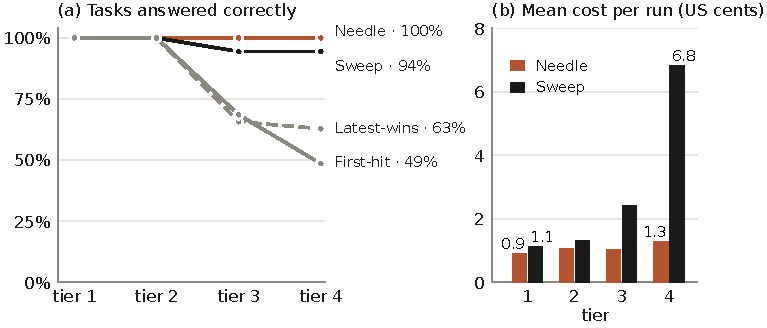
\includegraphics[width=\linewidth]{figures/results.pdf}
  \caption{Pilot results by tier. (a) Share of tasks answered correctly by Haiku 5.5 on needle tasks (39 runs per point) and sweep tasks (24 runs per point), with the two simulated reading policies on needle tasks for comparison. (b) Mean cost per run at API prices.}
  \label{fig:results}
\end{figure}

\begin{figure}[t]
  \centering
  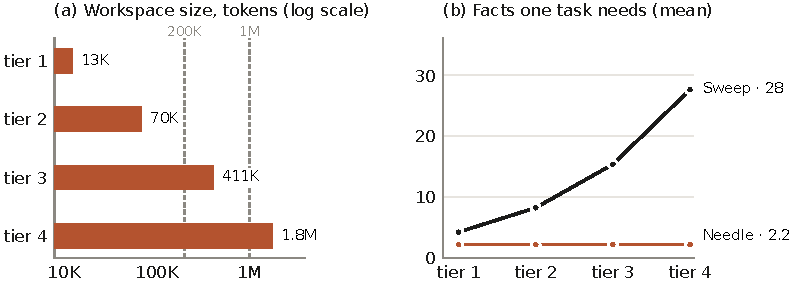
\includegraphics[width=\linewidth]{figures/tiers.pdf}
  \caption{What the tiers change. (a) Workspace size, with 200K and 1M tokens marked as two common context-window sizes. (b) Mean number of facts a task needs. Needle tasks need the same facts at every tier, and sweep tasks need more as clients and orders are added.}
  \label{fig:tiers}
\end{figure}

Table~\ref{tab:results} and Figure~\ref{fig:results} give the results. The model answered 155 of 156 needle runs correctly, a 95\% Wilson interval of 0.1\% to 3.5\% on its needle error rate. The interval treats the 156 runs as independent draws, although they are the same 39 questions asked at four tiers of one generated world, so it describes run-to-run variation in that world and says nothing about other seeds, personas or models. It answered 87 of 96 sweep runs correctly, with six misses at tier 3 and three at tier 4. The order of those two tiers is within noise, since five of the six tier-3 misses and all three tier-4 misses are on the late-payer questions, which have six runs per tier.

The structural measures predicted more difficulty than the agent met. By tier 4 a needle task had on average 5.5 stale statements of the facts it needs, the first-hit policy solved 49\% of needle tasks, and the latest-wins policy solved 67\%, while the agent solved all 39.

Size moved cost and not accuracy. The mean cost of a needle run rose from 0.9 to 1.3 cents between tiers 1 and 4 while the workspace grew by a factor of 141. The mean cost of a sweep run rose from 1.0 to 5.3 cents as the facts it needs rose from 4.3 to 27.6 (Figure~\ref{fig:tiers}b), which is between 0.10 and 0.25 cents per needed fact at every tier. For this model with search tools, cost tracked the evidence an answer requires far more closely than the files around it, a relation that rests on two kinds of question and is rough. The whole pilot cost \$3.89 at API prices.

\begin{table}[t]
  \caption{Pilot results for Claude Haiku 5.5 with file-search tools. Needle rows are 39 runs per tier and sweep rows are 24.}
  \label{tab:results}
  \centering
  \small
  \begin{tabular}{@{}llrrrr@{}}
    \toprule
    Scope & Measure & Tier 1 & Tier 2 & Tier 3 & Tier 4 \\
    \midrule
    Needle & Correct                & 39 of 39 & 39 of 39 & 38 of 39 & 39 of 39 \\
           & Mean turns             & 13.9 & 15.4 & 14.9 & 16.7 \\
           & Mean cost (cents)      & 0.9  & 1.0  & 1.1  & 1.3  \\
           & Facts needed (mean)    & 2.2  & 2.2  & 2.2  & 2.2  \\
    \midrule
    Sweep  & Correct                & 24 of 24 & 24 of 24 & 18 of 24 & 21 of 24 \\
           & Mean turns             & 19.2 & 20.0 & 20.0 & 34.5 \\
           & Mean cost (cents)      & 1.0  & 1.5  & 1.5  & 5.3  \\
           & Facts needed (mean)    & 4.3  & 8.3  & 15.4 & 27.6 \\
    \bottomrule
  \end{tabular}
\end{table}

\subsection{A source that lags: error analysis and ablation}
\label{sec:lag}

Eight of the ten wrong answers came from the two sweep questions that ask which clients paid an invoice after its final due date, five on the April question and three on the May question. Each of the eight is identical to the first predicted wrong answer for its task, the list of late payers computed from original due dates. At tiers 3 and 4 some due dates are extended by a one-line reply in the invoice thread (``New due date for INV-8918: June 15, 2026.''), which moves the date without resending the invoice. For such an invoice the original date is stated by the invoice email, its file copy in the drive, the tracker spreadsheet and the invoicing-app export, and the new date only by two emails in the thread.

\begin{table}[t]
  \caption{Runs that answered the late-payer sweep questions correctly at tiers 3 and 4 (two questions, two tiers, three trials). The first row is an earlier version of the same workspace with the same questions and keys. The third row deletes one folder from the second and changes nothing else.}
  \label{tab:lag}
  \centering
  \small
  \begin{tabular}{@{}lr@{}}
    \toprule
    Workspace & Correct \\
    \midrule
    Four sources (earlier version, no third-party apps) & 10 of 12 \\
    Eight sources                                       & 4 of 12 \\
    Eight sources with the invoicing export deleted     & 12 of 12 \\
    \bottomrule
  \end{tabular}
\end{table}

Table~\ref{tab:lag} gives the comparison. With the app exports present the model answered these questions correctly in 4 of 12 runs. We then deleted the invoicing export from the tier 3 and tier 4 workspaces, changed nothing else, and reran the same questions, and the model answered 12 of 12. Fisher's exact test against the unablated runs gives a two-sided $p = 0.001$, but the 12 runs in each arm are three repeats of four question-and-tier cells in one generated world and are not independent draws, so the test overstates the evidence. An export that lists every invoice with a due date is the shortest path to an answer about every client, and it presents itself as the system of record.

The export is a second copy of the old dates, and the first row of Table~\ref{tab:lag} shows that it is not their only carrier. The four-source version had no invoicing export, and 2 of its 12 runs gave the same wrong list as the eight-source misses on the same question and tier (the April question, once at tier 3 and once at tier 4). In both versions each invoice keeps the due date it was issued with, and the tracker spreadsheet lists the original date for most extended invoices, all 7 of the April and May invoices with an extension at tier 3 and 10 of the 15 at tier 4. The supported reading is therefore narrower than a single cause. Adding a second, authoritative-looking copy of an out-of-date fact went with a rise from 2 wrong runs in 12 to 8 in 12 across two versions of the dataset, and deleting that copy from the eight-source version left none.

Cost did not separate the wrong runs from the correct ones. Pooled over both tiers the eight wrong runs were cheaper, at a mean of 5.2 cents against 11.2, but that gap mostly reflects which tiers the runs fall in. At tier 3 the five wrong runs averaged 1.7 cents and the one correct run cost 1.3. At tier 4 the three wrong runs averaged 11.0 cents, including the costliest run of the pilot at 28.9 cents and 41 turns, against 14.5 cents for the three correct ones.

Two observations follow. A corrected invoice restates the record in full, so every system that receives it ends up current, and the agent's answers reflected corrections in all but one run. An extension changes one field in one place and nothing propagates it. The failure appeared only on sweeps, with a caveat about how often a needle question was exposed to it. On the needle questions that ask for one invoice's final due date the model was correct in 20 of 20 runs, but only 7 of those runs faced an export that showed a different date (3 at tier 3 and 4 at tier 4), and the 10 runs at tiers 1 and 2 had no export. Seven runs are consistent with the model reading the thread when a question concerns one client and reaching for the export when it concerns all of them, and they are too few to establish it. The remaining two errors were one superseded invoice total in a needle aggregate and one refund that was not subtracted in an order sweep.

\subsection{A container-build fault found by running the archive}
\label{sec:fault}

\begin{figure}[t]
  \centering
  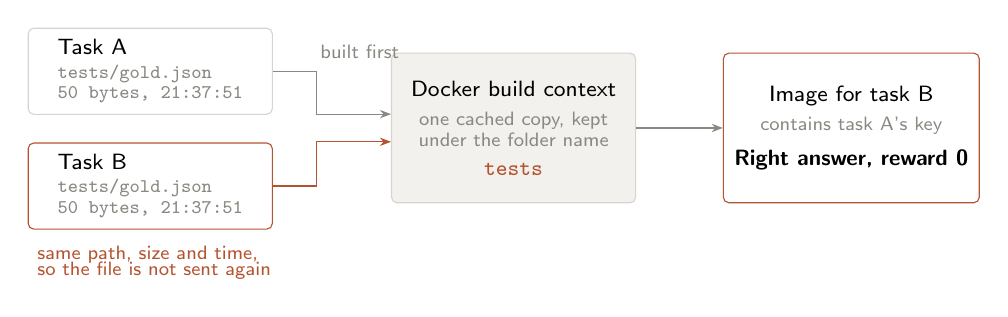
\begin{tikzpicture}[font=\sffamily\footnotesize, >={Stealth[length=4pt]},
      card/.style={draw=rule, rounded corners=2pt, minimum width=3.1cm, minimum height=1.05cm, align=left, inner sep=4pt},
      hot/.style={card, draw=accent}]
    \node[card] (a) {Task A\\[-1pt]{\scriptsize\ttfamily\color{faint}tests/gold.json}\\[-2pt]{\scriptsize\ttfamily\color{faint}50 bytes, 21:37:51}};
    \node[hot, below=0.35cm of a] (b) {Task B\\[-1pt]{\scriptsize\ttfamily\color{faint}tests/gold.json}\\[-2pt]{\scriptsize\ttfamily\color{faint}50 bytes, 21:37:51}};
    \node[card, fill=panel, minimum height=1.9cm, align=center, right=1.5cm of a, yshift=-0.72cm] (ctx) {Docker build context\\[1pt]{\scriptsize\color{faint}one cached copy, kept}\\[-2pt]{\scriptsize\color{faint}under the folder name}\\[1pt]{\ttfamily\color{accent}tests}};
    \node[hot, minimum height=1.9cm, align=center, right=1.1cm of ctx] (img) {Image for task B\\[1pt]{\scriptsize\color{faint}contains task A's key}\\[3pt]\textbf{Right answer, reward 0}};
    \draw[->, faint] (a.east) -- ++(0.55,0) |- node[pos=0.0, above right, font=\sffamily\scriptsize, text=faint, yshift=1pt, xshift=-2pt] {built first} ([yshift=5pt]ctx.west);
    \draw[->, accent] (b.east) -- ++(0.55,0) |- ([yshift=-5pt]ctx.west);
    \node[font=\sffamily\scriptsize, text=accent, align=left, below=0.08cm of b.south west, anchor=north west] {same path, size and time,\\[-2pt]so the file is not sent again};
    \draw[->, faint] (ctx) -- (img);
  \end{tikzpicture}
  \caption{How a task came to be graded with another task's key. Two tasks hold a same-named key file of equal size and whole-second timestamp in folders that are both called \code{tests}. In the first archive the key files of one tier share one timestamp, 21:37:51 Pacific time at tiers 1 to 3 and 21:37:52 at tier 4. The builder reuses the first task's copy when it builds the second task's verifier image.}
  \label{fig:fault}
\end{figure}

The first archive we published, of an earlier four-source version with 164 tasks, passed every gate then in place, including oracle and no-op runs made from the build folder. When we unpacked the published archive and ran it as a reader would, the oracle wrote the correct answer and still scored zero on 31 of 105 needle tasks at tiers 2 to 4. The verifier's per-field output showed each affected trial had been compared with the key of a different task in the same family.

The cause is in the container build (Figure~\ref{fig:fault}). With Docker 28.0.4 and buildx 0.22.0, the builder reused a file from an earlier build whose context folder had the same name whenever the file's path, size and modification time all matched. Harbor builds each task's \code{tests} folder as the verifier image, every task names that folder \code{tests}, keys within a task family are often the same size, and unpacking an archive sets whole-second timestamps. A minimal reproduction with two folders named \code{tests}, each holding a 16-byte \code{gold.json} with different content and equal timestamps, produced two images that both contained the first file. Giving the two folders different names, or the two files different names, removed the effect. Runs from the build folder had not shown it because the files there carried distinct sub-second timestamps.

The fix is to make any file that differs between tasks and sits in a build context carry a hash of its content in its name (for example \code{gold.737da39abb37.json}), so that two tasks share a path only when they share the file. The verifier also checks the key against the hash in its name and exits with an error on a mismatch, which a harness reports as a failed verification. A unit test asserts the naming rule across tiers. After the change, the oracle scored 1.0 and the no-op agent 0.0 on every task run from an unpacked copy of the archive, for that version and for the 188 tasks of the current one.

We also added a static check to a small open-source reader for Harbor tasks.\footnote{\url{https://github.com/nbdesai1992/harbor-inspect}} It flags any file that a build copies in and that shares a path and size with a different file in another scanned task. It flags 135 of the 164 tasks in the first archive, none in the corrected one, and none of 136 public tasks from three datasets, all of which use a shared verifier and therefore do not build a \code{tests} image. The failure is silent and is not specific to this generator. Any dataset with a per-task verifier image and fixed-name fixture files is exposed to it once file timestamps coincide.

\section{Limitations}

The pilot uses one persona, one seed, one small model and one harness, with a single trial per needle task and three per sweep task, so it supports statements about where errors appeared and only rough statements about rates. Repeated runs of one question in one generated world are not independent samples of workspaces, so the interval and the exact test above describe run-to-run variation in this world only. There is no human baseline for these questions. The comparison with the four-source version in Table~\ref{tab:lag} is across dataset versions, and the ablation in the same table is the controlled one. The agent had search tools, and no run had to fit a workspace into its context window. A model without tools, or one asked to read a tier-4 workspace in context, would face a different problem. Text is rendered from templates with a voice profile, which makes it cleaner than real mail. Tasks are read-only, so nothing here measures side effects such as sending a message or moving a meeting. Both personas share one engagement-cycle engine, and only one kind of system-of-record lag is planted, beside the tracker rows that are left at superseded values. Sources are files in a sandbox, and the same world could be served through tool interfaces. Finally, the tiers remain uncalibrated. The correct next step is the one the literature recommends, which is to define a tier by a reference solver's pass rate.

\section{Conclusion}

Drawing final facts independently of the complexity tier gives a clean experimental variable, since the same question with the same key can be asked of workspaces that differ by two orders of magnitude in size and in the number of systems that hold a copy of each fact. Used on our own tiers, that variable showed that volume raised an agent's cost roughly in step with the evidence an answer needs and hardly touched its accuracy. What did reduce accuracy was an out-of-date fact repeated by a source that looked authoritative. Removing that source removed the errors in this workspace, and the same error had appeared at a lower rate in a version that never had the source. For environment builders the pilot suggests that planted, labelled disagreement between systems is a more effective difficulty control than volume. The broader lesson concerns checking. The packaging fault that mattered most was invisible to every in-process gate and to a harness run from the build folder, and appeared only when the published archive was unpacked and run.

\paragraph{Availability.} The 188 tasks are available as a single archive at \url{https://nealdes.ai/assets/orbifex/cpa-solo-harbor-v2.tar.gz}, the earlier four-source version at \url{https://nealdes.ai/assets/orbifex/cpa-solo-harbor.tar.gz}, and an illustrated summary at \url{https://nealdes.ai/articles/persona-to-environment}.

\begin{thebibliography}{10}

\bibitem{wildawm}
Wang et~al.
\newblock Agent World Model in the Wild: Computer-Use Agent Environment Synthesis.
\newblock arXiv:2610.26828, 2026.

\bibitem{mypcbench}
Jang, Jang, Koh, and Salakhutdinov.
\newblock MyPCBench: A Benchmark for Personally Intelligent Computer-Use Agents.
\newblock arXiv:2606.16748, 2026.

\bibitem{anchor}
Rana and Ivanov.
\newblock Anchor: Preventing Artifact Drift for Reliable Agent Verification.
\newblock arXiv:2605.26321, 2026.

\bibitem{enterprisebench}
Enterprise-Bench.
\newblock L1-L2 suite, version 2, dataset README.
\newblock Harbor registry, read November 14, 2026. \url{https://hub.harborframework.com/}.

\bibitem{emailbench}
Singh et~al.
\newblock EmailBench: A Benchmark for Evaluating LLM Agents on Enterprise Email and Productivity Tasks.
\newblock arXiv:2609.31906, 2026.

\bibitem{generalagent}
M.~Senghaas.
\newblock General Agent: A Self-Evolving, Synthetic Agent Environment.
\newblock Prime Intellect, May 18, 2026. \url{https://primeintellect.ai/blog/general-agent}.

\bibitem{grads}
Yang et~al.
\newblock GRADS: Graph-Regulated Agentic Data Synthesis with Controllable Difficulty.
\newblock arXiv:2610.21167, 2026.

\bibitem{benchjack}
Wang, Li, Mang, Cheung, Sen, and Song.
\newblock Do Androids Dream of Breaking the Game? Systematically Auditing AI Agent Benchmarks with BenchJack.
\newblock arXiv:2605.12673, 2026.

\bibitem{hackerfixer}
Zhong, Segal, Bercovich, Saxena, Zhang, and Raghunathan.
\newblock Hardening Agent Benchmarks with Adversarial Hacker-Fixer Loops.
\newblock arXiv:2606.08960, 2026.

\bibitem{harbor}
Harbor.
\newblock Release 0.26.0 and documentation, November 13, 2026.
\newblock \url{https://github.com/harbor-framework/harbor}.

\end{thebibliography}

\end{document}
